\section{Лекция 4 -- 2024-03-15 -- Закон распределения времени пребываения в
подмножестве состояний}

\begin{ex}
  Рассмотрим следующую марковскую цепь:
  $\mathcal{S} = \left\{ S_0, S_1, \dots, S_m \right\} $.
  $\xi(0) = 0 \leftrightarrow \bar{p}(0) = (1, 0, \dots, 0)^T$.

  Обозначим $T_U$ -- время до первого выхода из $U = \left\{ S_0 \right\} $.

  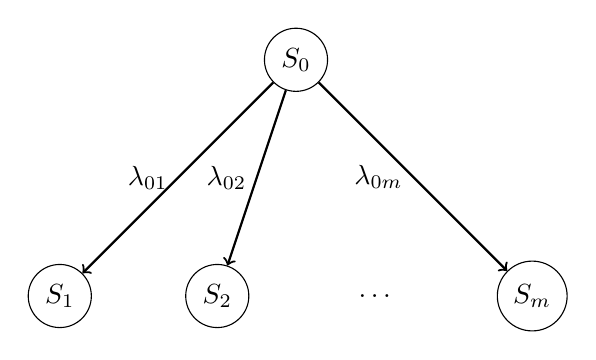
\begin{tikzpicture}
    \begin{scope}[every node/.style={fill=white,circle,draw=black}]
      \node (S_0) at (1,0) {$S_0$};
      \node (S_1) at (-2,-3) {$S_1$};
      \node (S_2) at (0,-3) {$S_2$};
      \node[draw=white] (S_dots) at (2, -3) {$\dots$};
      \node (S_m) at (4,-3) {$S_m$};
    \end{scope}

    \begin{scope}[->, every edge/.style={draw=black,thick}]
      \path (S_0) edge node[left] {$\lambda_{01}$} (S_1);
      \path (S_0) edge node[left] {$\lambda_{02}$} (S_2);
      \path (S_0) edge node[left] {$\lambda_{0m}$} (S_m);  
    \end{scope}
  \end{tikzpicture}

  В этом случае вероятность нахождения в нулевом состоянии будет определяться
  дифференциальным уравнением:
  \[
    \begin{cases}
      p_0'(t) = - \left( \sum\limits_{k=1}^m \lambda_{0k} \right) p_0(t), \\
      p_0(0) = 1,
    \end{cases}
  \]
  которое, как несложно заметить, не зависит от того как между собой переходят 
  все остальные состояния.

  Функция распределения, по определению:
  \[
    F_{T_U} (t) = P(T_U < t) = 1 - P(T_U \geqslant t) = 1- p_0(t).
  \]
  -- эта функция распределения также не зависит от никаких других 
  интенсивностей переходов. Продифференцируем, чтобы получить плотность распределения:
  \[
    p_{T_U}(t) = - p_0'(t) = \left( \lambda(t) e^{ - \int_0^t \lambda(\tau) d\tau } \right)'
  \]

  Здесь есть очень важный частный случай, когда $\lambda = \sum_{k=1}^m \lambda_{0k} = \operatorname{const}(t)$ -- случай однородной марковской цепи (ну не только когда вся цепь однородная, достаточно просто однородности исходящих из нулевого состояния интенсивностей):
  \[
    p_{T_U}(t) = \lambda e^{-\lambda t}
  \]
  -- показательный закон с параметром $\lambda$. В этом случае легко посчитать
  математическое ожидание времени выхода: $MT_U = \dfrac{1}{\lambda}$.
\end{ex}

\begin{ex}
  Рассмотрим пример, в котором дано: $p_{T_U}(t) = \alpha^2 t e^{-\alpha t}$
  (как и в предыдущем примере $U = \left\{ S_0 \right\} $). Найдём
  тогда $\lambda(t)$.
  \[
    F_{T_U}(t) = \int\limits_0^t \alpha^2 \tau e^{-\alpha \tau} \, d\tau
    = 1 - e^{-\alpha t} - \alpha t e^{-\alpha t}.
  \]
  \[
    p_0(t) = 1 - F_{T_U}(t) = e^{-\alpha t} + \alpha t e^{-\alpha t}.
  \]
  \[
    \lambda(t) = - \dfrac{p_0'(t)}{p_0(t)}
    = - \dfrac{-\alpha e^{-\alpha t} + \alpha e^{-\alpha t} - \alpha^2 t e^{-\alpha t}}{e^{-\alpha t}+ \alpha t e^{-\alpha t}}
    = \dfrac{\alpha^2 t}{1+ \alpha t}.
  \]
\end{ex}

\begin{ex}
  Рассмотрим вот такую марковскую цепочечку:

  \begin{figure}[h!]
    \centering
    \begin{tikzpicture}
      \begin{scope}[every node/.style={fill=white,circle,draw=black}]
          \node (S_1) at (0,0) {$S_1$};
          \node (S_2) at (2,0) {$S_2$};
          \node[draw=white,rectangle] (S_dots_1) at (4,0) {$\dots$};
          \node (S_m) at (6,0) {$S_m$};

          \node (S_{m+1}) at (0,-3) {$S_{m+1}$};
          \node (S_{m+2}) at (2,-3) {$S_{m+2}$};
          \node[draw=white,rectangle] (S_dots_2) at (4,-3) {$\dots$};
          \node (S_{m+r}) at (6,-3) {$S_{m+r}$};
      \end{scope}
    
      \begin{scope}[->, every edge/.style={draw=black,thick}]
        \path (S_1) edge [bend right=30] node[left] {} (S_2);
        \path (S_2) edge [bend right=30] node[left] {} (S_1);
        \path (S_2) edge [bend right=30] node[left] {} (S_dots_1);
        \path (S_dots_1) edge [bend right=30] node[left] {} (S_2);
        \path (S_dots_1) edge [bend right=30] node[left] {} (S_m);
        \path (S_m) edge [bend right=30] node[left] {} (S_dots_1);

        \path (S_1) edge  node[left] {} (S_{m+1});
        \path (S_2) edge  node[left] {} (S_{m+2});
        \path (S_m) edge  node[left] {} (S_{m+2});
        \path (S_m) edge  node[left] {} (S_{m+r});
      \end{scope}

      \node[draw=black,very thick,dotted,fit=(S_1) (S_m)] (FIt1) [acateur][label=left:{$U$}]{};
    \end{tikzpicture}
  \end{figure}

  Тогда у нас множество состояний $\mathcal{S} = \left\{ S_i | i=\overline{1, m+r} \right\} $,
  подмножество $U = \left\{ S_1, S_2, \dots, S_{m} \right\}, m < m+r $, 
  a $\bar{p}(0)^T = ( \underbrace{\dots}_{\text{не нули}},
  \underbrace{0, 0, \dots, 0}_{\text{нули}})$ (начинаем где-то внутри $U$). 

  Обозначим $T_U$ -- время однократного пребывания в $U$.

  \[
    \begin{cases}
      p_1' = - \sum_{k=2}^{m+2} \lambda_{1k} p_1 + \sum_{k=2}^m \lambda_{k 1} p_k  \\
      p_m' = - \left( \sum_{k=1, k\neq m}^{m+r} \lambda_{mk} \right) p_m + \sum_{k=1}^m \lambda_{km} p_k \\
      p_{m+1}' = \sum_{k=1}^m \lambda_{k, m+1} p_k \\
      p_{m+r}' = \sum_{k=1}^m \lambda_{k, m+r}^{m} \lambda_{k, m+r} p_k.
    \end{cases}
  \]

  Функция распределения, по определению будет равна:
  \[
    F_{T_U}(t) = P(T_U < t) = 1 - P(T_U \geqslant t)
    = 1 - \sum_{k=1}^m p_k(t)
    = \sum_{k=m+1}^{m+r} p_k(t).
  \]

  Дифференцированием получаем:
  \[
    p_{T_U}(t) = \sum_{k=m+1}^{m+r} p_k'(t)
    = \sum_{k=m+1}^{m+r} \sum_{j=1}^m \lambda_{k, j} p_j
    = \sum_{j=1}^m \left( \sum_{k=m+1}^{m+r} \lambda_{jk} p_j \right)
    = \sum_{j=1}^m \left( \sum_{k=m+1}^{m+r} \lambda_{jk} \right) p_j
  \]
\end{ex}

\begin{ex}
  Пусть для однородной марковской цепи со счетным количеством состояний 
  $p(0)^T = (1, 0, \dots)$, интенсивности на рисунке.
  Найти закон распределения времени появления третьей особи.
  \begin{figure}[h!]
    \centering
    \begin{tikzpicture}
      \begin{scope}[every node/.style={fill=white,circle,draw=black}]
        \node (S_1) at (0,0) {$S_1$};
        \node (S_2) at (2,0) {$S_2$};
        \node (S_3) at (4,0) {$S_3$};
        \node[draw=white] (S_dots) at (6,0) {$\dots$};
      \end{scope}
    
      \begin{scope}[->, every edge/.style={draw=black,thick}]
        \path (S_1) edge [bend right=30] node[below] {$\lambda$} (S_2);
        \path (S_2) edge [bend right=30] node[below] {$2\lambda$} (S_3);
        \path (S_3) edge [bend right=30] node[below] {$3\lambda$} (S_dots);
      \end{scope}
      \node[draw=black,very thick,dotted,fit=(S_1) (S_2)] (FIt1) [acateur][label=left:{$U$}]{};
    \end{tikzpicture}
  \end{figure}

  \[
    \begin{cases}
      p_1' = - \lambda p_1, \\
      p_2' = -2 \lambda p_2 + \lambda p_1.
    \end{cases}
    \Rightarrow
    \begin{cases}
      s \tilde{p_1} - 1 = - \lambda \tilde p_1, \\
      s \tilde p_2 = - 2 \lambda \tilde p_2 + \lambda \tilde p_1.
    \end{cases}
    \Rightarrow
    \begin{cases}
      \tilde p_1 = \dfrac{1}{s+\lambda} \risingdotseq e^{-\lambda t}, \\
      \tilde p_2 = \dfrac{\lambda \tilde p_1}{s+2\lambda} 
      = \dfrac{1}{(s+\lambda)(s+2\lambda)} \risingdotseq e^{-\lambda t} - e^{-2\lambda t}.
    \end{cases}
  \]

  Тогда:
  \[
    p_{T_U} (t) = 2\lambda p_2(t) = 2\lambda e^{-2\lambda t} - 2\lambda e^{-2\lambda t}
    = 2 \lambda e^{-\lambda t} - 1 \cdot 2\lambda e^{-2\lambda t}
  \]
  -- смесь двух показательных законов.
  Тогда так как это показательные законы, очень легко можно получить матожидание:
  \[
    MT_U = \dfrac{2}{\lambda} - \dfrac{1}{2\lambda} = \dfrac{3}{2\lambda}.
  \]
\end{ex}



\subsection{Прямые и обратные уравнения Колмогорова}

\begin{definition}
  Пусть $\xi_t$ -- однородная марковская цепь,
  $P(\xi_{t+\Delta t} = j | \xi_t = i) = \lambda_{ij} \Delta t + o(\Delta t)$.
  $p_{ij}(t) = (\xi_t = j | \xi_0 = i)$ -- переходные вероятности за $t$,
  тогда $P(t) = (p_{ij}(t))$ -- матрица переходных вероятностей.
\end{definition}

\begin{theorem}
  Для однородной марковской цепи

  Если $P(t)$ -- матрица переходных вероятностей однородной марковской цепи.
  $\bar{p}(0)$ -- вектор вероятностей начальных состояний, то
  \[
    \bar{p}(t)^T = \bar{p}(0)^T \cdot P(t)
  \]
\end{theorem}
\begin{proof}
  \[
    p_j(t) = P(\xi_t = j) = \sum_{k=1}^m P(\xi_t = j | \xi_0=j) P(\xi_0=k)
    = \sum_{k=1}^m p_{kj}(t) p_k(0)
  \]
\end{proof}

Мораль: если бы мы знали матрицу переходных вероятностей, не надо было бы 
решать систему диффуров, просто можно было бы умножить эту матрицу на столбец
начальных вероятностей.

\begin{corollary}
  \[
    \bar{p}'(t) = \bar{p}(0)^T \cdot P'(t)
  \]

  С другой стороны, для однородной цепи:
  \[
    \bar{p}'(t)^T = \bar{p}(t)^T \cdot \Lambda = \bar{p}(0)^T \cdot P(t) \cdot \Lambda
  \]

  Следовательно, 
  \[
    P'(t) = P(t) \cdot \Lambda
  \]
  -- система прямых уравнений Колмогорова.

  Чуть сложнее, но можно доказать и такое:
  \[
    P'(t) = \Lambda \cdot P(t)
  \]
  -- система обратных уравнений Колмогорова.
\end{corollary}

\begin{ex}
  Запишем прямую и обратную системы уравнений Колмогорова для цепи:
  \begin{figure}[h!]
    \centering
    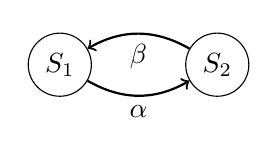
\begin{tikzpicture}
      \begin{scope}[every node/.style={fill=white,circle,draw=black}]
        \node (S_1) at (1,0) {$S_1$};
        \node (S_2) at (3,0) {$S_2$};
      \end{scope}
    
      \begin{scope}[->, every edge/.style={draw=black,thick}]
        \path (S_1) edge [bend right=30] node[below] {$\alpha$} (S_2);
        \path (S_2) edge [bend right=30] node[below] {$\beta$} (S_1);
      \end{scope}
    \end{tikzpicture}
  \end{figure}
  \[
    \Lambda = \begin{pmatrix}
      -\alpha & \alpha \\
      \beta & - \beta
    \end{pmatrix} 
  \]

  Прямая система:
  \[
    \begin{cases}
      p_{11}' = - \alpha p_{11} + \beta p_{12} \\
      p_{12}' = \alpha p_{11} - \beta p_{12} \\
      p_{21}' = -\alpha p_{21} + \beta p_{22} \\
      p_{22}' = \alpha p_{21} - \beta p_{22}.
    \end{cases}
  \]

  Обратная система (в некотором смысле, она важнее):
  \[
    \begin{cases}
      p_{11}' = - \alpha p_{11} + \alpha p_{21}, \\
      p_{12}' = -\alpha p_{12} + \alpha p_{22}, \\
      p_{21}' = \beta p_{11} - \beta p_{21}, \\
      p_{22}' = \beta p_{12} - \beta p_{22}.
    \end{cases}
  \]
\end{ex}

\subsection{Способы решения}

\begin{enumerate}
  \item Операционное решение -- не интересно, уже знаем.
  \item Матричная экспонента:
    \[
      \begin{cases}
        P'(t) = \Lambda \cdot P(t), \\
        P(0) = E.
      \end{cases}
      \Rightarrow
      P(t) = E \cdot e^{\Lambda t} = \sum_{k=0}^\infty \dfrac{(\Lambda t)^k}{k!}
    \]
  \item Численно
\end{enumerate}

\begin{corollary}
  \[
    P'(0) = \Lambda \cdot P(0) = \Lambda
    \Rightarrow
    \lambda_{ij} = p_{ij}' (0)
  \]
\end{corollary}

Впечатляет? -- тишина -- ой, ладно, только я в своём преклонном возрасте умею впечатляться.

\begin{ex}
  % TODO рисунок
  \[
    \Lambda = \begin{pmatrix}
      -\alpha & \alpha \\
      \beta & -\beta
    \end{pmatrix} 
  \]

  \[
    \Lambda = U \cdot D \cdot U^{-1}
    = \dfrac{1}{\alpha+\beta} \begin{pmatrix}
      1 & -\alpha \\
      1 & \beta
    \end{pmatrix}  \cdot \begin{pmatrix}
      0 & 0 \\
      0 & - (\alpha+\beta)
    \end{pmatrix} \cdot \begin{pmatrix}
      \beta & \alpha \\
      -1 & 1
    \end{pmatrix} 
  \]

  \[
    \Lambda^k = \dfrac{1}{\alpha+\beta} \begin{pmatrix}
      1 & -\alpha \\
      1 & \beta
    \end{pmatrix} \cdot \begin{pmatrix}
      0 & 0 \\
      0 & (-\alpha-\beta)^k
    \end{pmatrix} \cdot \begin{pmatrix}
      \beta & \alpha \\
      -1 & 1
    \end{pmatrix} 
  \]

  \[
    P(t) = e^{\Lambda t} = \sum_{k=0}^\infty \dfrac{(\Lambda t)^k}{k!}
    = \dfrac{1}{\alpha+\beta} \begin{pmatrix}
      1 & -\alpha \\
      1 & \beta
    \end{pmatrix}  \cdot
    \sum_{k=0}^\infty \dfrac{D^k t^k}{k!} \cdot
    \begin{pmatrix}
      \beta & \alpha \\
      -1 & 1
    \end{pmatrix} = \dots = \dfrac{1}{\alpha+\beta} \begin{pmatrix}
      1 & -\alpha \\
      1 & \beta
    \end{pmatrix}  \cdot
    \begin{pmatrix}
      1 & 0 \\
      0 & e^{-(\alpha+\beta) t}
    \end{pmatrix} \cdot \begin{pmatrix}
      \beta & \alpha \\
      -1 & 1
    \end{pmatrix} 
  \]

  \[
    P(t) = e^{\Lambda t} = 
  \]

  Можно было не находить собственные вектора, т.к. зная общий вид
  степени, можно было бы воспользоваться методом неопределённых коэффициентов:
  представить $p_{ij}(t)$ в виде $A + B e^{-(\alpha+\beta) t}$, и найти 
  эти коэффициенты из условий: $p_{ij}(0) = 0, p_{ij}'(0) = \lambda_{ij}$.
\end{ex}

\begin{definition}
  Если $ \forall i : \exists \lim_{t\to +\infty} p_{ij}(t) = \pi_j, 0 < \pi_j < 1, \sum \pi_j = 1$,
  то цепь называется \emph{эргодической}.
\end{definition}

\begin{theorem}[эргодическая]
  Пусть $\mathbb{S} = \left\{ S_1, S_2, \dots, S_m, \dots \right\} $ --
  марковская цепь со счетным множеством состояний. Если
  \[
    \exists S_{j_0} \exists h>0 \exists \delta \in(0, 1], \forall S_i \in \mathbf{S} : P_{ij_0}(h) \geqslant \delta,
  \]
  тогда цепь эргодична, причём $|p_{ij}(t) - \pi_j| \leqslant (1-\delta)^{\left[\dfrac{t}{h}\right]}$
\end{theorem}

\begin{corollary}
  В условиях эргодической теоремы:
  \begin{enumerate}
    \item $\exists \lim_{t\to +\infty} p_j(t) = \pi_j$, причём легко показать, 
      что
      \[
        |p_j(t) - \pi_j| = |\sum_{k} p_k(0) p_{kj}(t) - \sum_{k} \pi_j p_{k}(0)|
        \leqslant |\sum_k p_k(0) \left( p_{kj}(t) - \pi_j \right) |
        \leqslant (1-\delta)^{ \left[ \dfrac{t}{h} \right] } \cancel{\sum_{k} p_k(0)}
      \]
  \end{enumerate}
\end{corollary}
